
\chapter{Výsledky práce}

V tejto kapitole zhrnieme výsledky, ktoré naša práca dosiahla.

Už v predchádzajúcich kapitolách sme sa stretli s niekoľkými príkladmi, napríklad ako si
program poradil s vkladaíim do hairpinu - obrázok \ref{obr:insert_circle_hairpin}.

Na ďalšom (obrázok \ref{obr:delete_insert_multibranch}) simulujeme mazanie s následným vkladaním,
teda 2 k sebe inverzne operácie. Po zmazaní bázových párov na hornej vetve molekuly, sa nám všetky
nepárové bázy zliali a vytvorili jednu loop. Následne po opätovnom vložení bázovych parov (pre lepsie
zviditelnenie sme ich označili "I"), vzniklá štruktúra veľmi podobná predchádzajúcej.

Obrázok má za cieľ ukázať, že vieme znovu nakresliť pôvodnu štruktúru iba s malými zmenamy v pozícií
nukleotidov (výsledne loopy sú trochu plytšie ako pôvodne).

Rovnako obrázok \ref{obr:delete_insert_multibranch_loop} rekonštruuje vetvenie sa stromu. Ako je vidieť,
v tomto obrázku je už viac rozdielov, vychylenie je celkom badatelné.

Na takto malých častiach bez velkých vetvení nam ani taketo zmeny nevadia. Pri velkych molekulach
ako ukazeme neskor problemy nastavaju.

\begin{figure}[H]
  \begin{subfigure}{0.3\textwidth}
%trim=left bottom right top
    \includegraphics[clip, trim=1cm 21cm 14cm 2.5cm, width=0.85\textwidth]{../img/alg/insert/2/multibranch-beg}
  \end{subfigure}
  \begin{subfigure}{0.3\textwidth}
%trim=left bottom right top
    \includegraphics[clip, trim=1cm 21cm 14cm 2.5cm, width=0.85\textwidth]{../img/alg/insert/2/multibranch-del}
  \end{subfigure}
  \begin{subfigure}{0.3\textwidth}
%trim=left bottom right top
    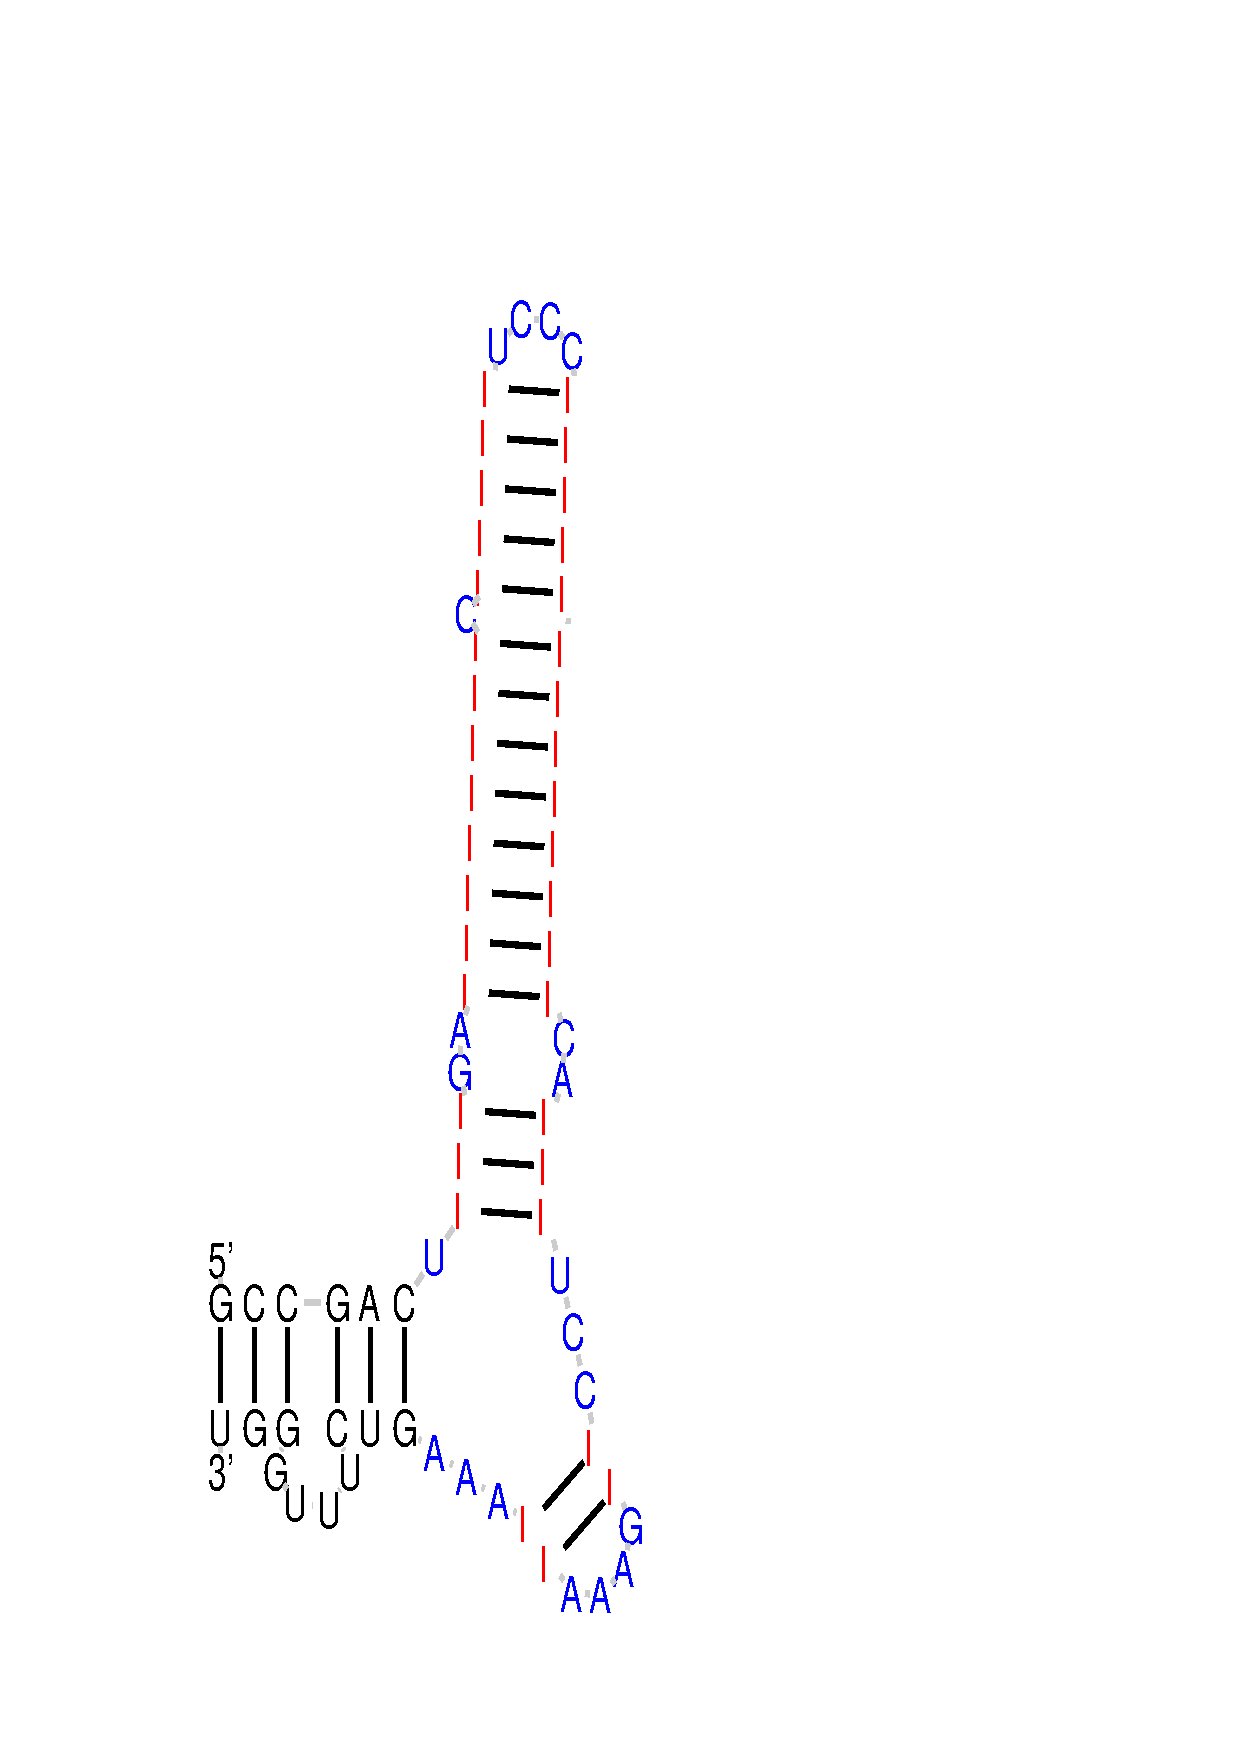
\includegraphics[clip, trim=1cm 21cm 14cm 2.5cm, width=0.85\textwidth]{../img/alg/insert/2/multibranch-del-ins}
  \end{subfigure}
  \caption{Inverzne operacie: rekonštrukcia stemu}
  \label{obr:delete_insert_multibranch}
\end{figure}


\begin{figure}[H]
  \begin{subfigure}{0.3\textwidth}
%trim=left bottom right top
    \includegraphics[clip, trim=1cm 21cm 14cm 2.5cm, width=0.85\textwidth]{../img/alg/insert/3/multibranch-beg}
  \end{subfigure}
  \begin{subfigure}{0.3\textwidth}
%trim=left bottom right top
    \includegraphics[clip, trim=0 0 0 15cm, width=0.85\textwidth]{../img/alg/insert/3/multibranch-del}
  \end{subfigure}
  \begin{subfigure}{0.3\textwidth}
%trim=left bottom right top
    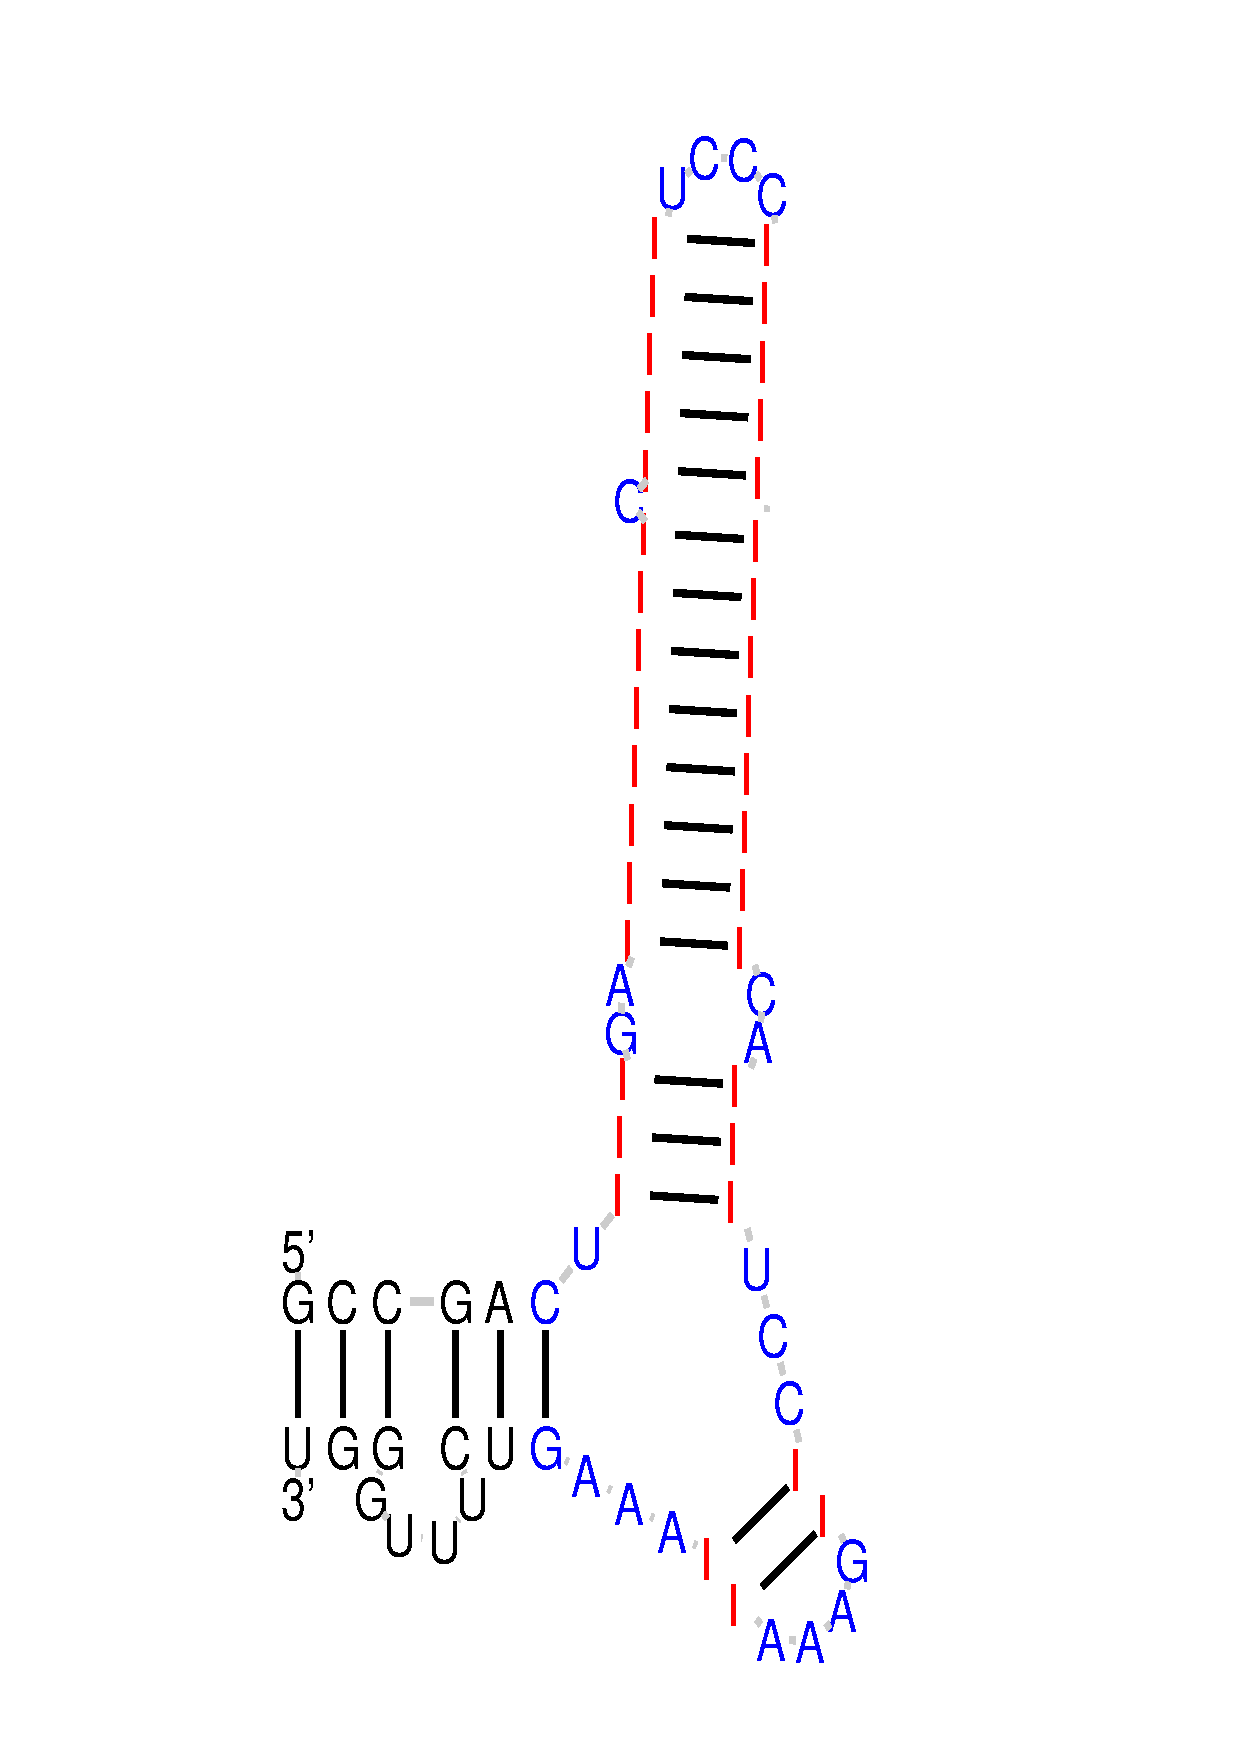
\includegraphics[clip, trim=0 0 0 2cm, width=0.85\textwidth]{../img/alg/insert/3/multibranch-del-ins}
  \end{subfigure}
  \caption{Inverzné operácie: rekonštrukcia multibranch loop}
  \label{obr:delete_insert_multibranch_loop}
\end{figure}


Ako ďalšie, testovali sme schopnosť nášho algoritmu vizualizovať známu podjednotku 16S ribozomálnej RNA
na živočisnej ríši. CRW databáza obsahuje 16 organizmov so známou sekundárnou štruktúrou.

Ribozomálna RNA bola vybrata lebo je v centre záujmu mnohých výskumov a taktiež kvôli jej veľkosti
a zložitosti.

Náš vizualizačný test sme spustili na všetky páry RNA, z ktorých sme získali 256 vizualizácií.

%Na začiatku potrebujeme uviesť, že z celkového pocčtu 256 vizualizácií dopadlo 21 neúspechom pre rôzne dôvody.
%Tým hlavným je 

Na obrázku \ref{obr:statistika_prekryvy} vidíme počty molekúl s daným počtom prekryvov. 
Je ale niekoľko typov molekul, u ktorých sme nejaké prekryvy čakali - napríklad, ak sme v nej
potrebovali prekresliť multibranch loop. Takúto závislosť nám vyjadrujú ďalšie dva grafy,
prvý - \ref{obr:statistika_prekryvy_s_rotaciami} nám ukazuje, že ak program musel rotovať
a prekreslovať multibranch loopy, nedarilo sa mu najlepšie. Naopak, ak z prvého grafu
odoberieme molekuly, ktoré museli použiť rotácie - graf \ref{obr:statistika_prekryvy_bez_rotacii},
vidíme, že algoritmus šablonovej vizualizácie si viedol celkom dobré, prekryvy vznikali iba ojedinele.


\begin{figure}
  \includegraphics[width=1\textwidth]{../img/statistika/prekryvy-pocetmolekul}
  \caption{Počet prekryvov v testovaných molekulách}
  \label{obr:statistika_prekryvy}
\end{figure}


\begin{figure}
  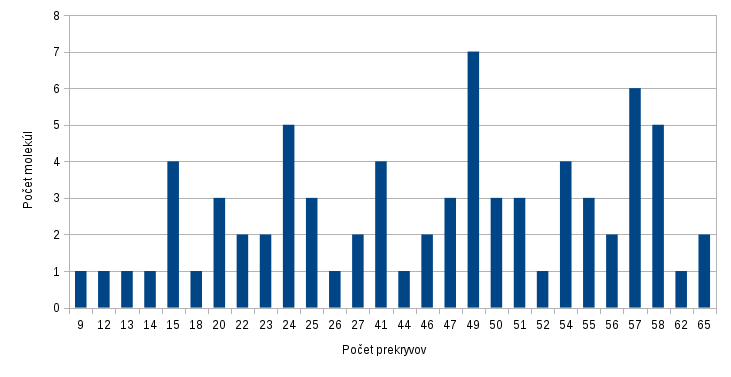
\includegraphics[width=1\textwidth]{../img/statistika/prekryvy-pocetmolekul-s-rotaciami}
  \caption{Počet prekryvov: molekuly, ktoré potrebovali prekreslit multibranch loop}
  \label{obr:statistika_prekryvy_bez_rotácii}
\end{figure}


\begin{figure}
  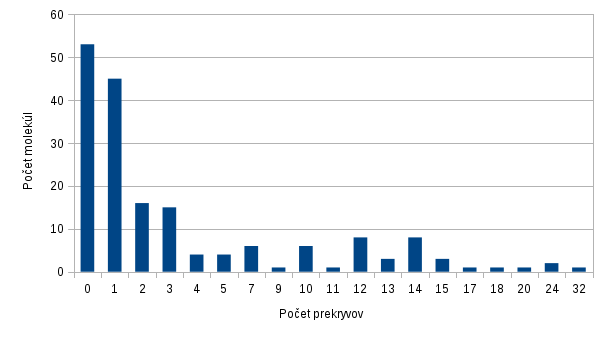
\includegraphics[width=1\textwidth]{../img/statistika/prekryvy-pocetmolekul-bez-rotacii}
  \caption{Počet prekryvov: molekuly bez prekreslovania multibranch loop}
  \label{obr:statistika_prekryvy_s_rotaciami}
\end{figure}

\begin{table}[b]
  \centering
  \begin{tabular}{l@{\hspace{1.5cm}}D{.}{,}{3.2}D{.}{,}{1.2}D{.}{,}{2.3}}
    \toprule
                                  & \mc{\textbf{Počet}}               & \mc{\textbf{Smerodajná}}    & \\
    \mc{\textbf{Vzdialenosť}}     & \mc{\textbf{prekryvov}}           & \mc{\textbf{odchýlka}}      & \\
                                  & \mc{\textbf{(priemer)}}           &                             & \\
    \midrule
    1.                            & 5.13                              & 1.64                        & \\
    5.                            & 13.38                             & 9.57                        & \\
    10.                           & 14.13                             & 12.47                       & \\
    15.                           & 15.25                             & 0.66                        & \\
    \bottomrule
  \end{tabular}
\caption{Počty prekryvov v závislosti od tree-edit-distance vzdialenosti}
\label{tab:statistika_prekryvy}
\end{table}

Z tabuľky \ref{tab:statistika_prekryvy} je vidieť, že počet prekryvov závisí od počtu operacií vkladania
a mazania ktoré v molekule musíme urobiť. Štatistika pracuje s prvou, piatou, desiatou a pätnástou najbližšou
molekulou z pohľadu $tree-edit-distance$.

Zaujímavosťou je, že ako najvzdialenejšiu molekulu (v poradí pätnástu) si všetci vybrali molekulu od
jedného konkrétneho zástupcu $echinococcus\_granulosus$ a vzdialenosť je $805,63$ s odchylkou $12,92$.

\section{Celkové výsledky}

V tejto kapitole uvedieme vygenerované obrázky niektorých molekúl a na nich ukážeme časté problémy,
ktoré pri vizualizácii nastavali.

\subsection{Otáčanie vetvy kvôli existujúcej hrane}

Jedným príkladom za všetky je molekula žívočícha $Tripedalia cystophora$ - meduzy.
Po tom, čo sme dali molekulu nakresliť samu na seba vznikol problém, že celá jedna
vetva molekuly sa otočila na jednu stranu. Je to spôsobene existenciou bázového páru,
ktorý je v pôvodnej molekule znázornený dlhšou lomenou čiarou.

Keďže nás program všetky vzdialenosti normalizuje a následne ukladá bázy stemu na jednu priamku,
vznikajú obrázky podobné \ref{obr:chyba_otočenie_vetvy}.

\begin{figure}
  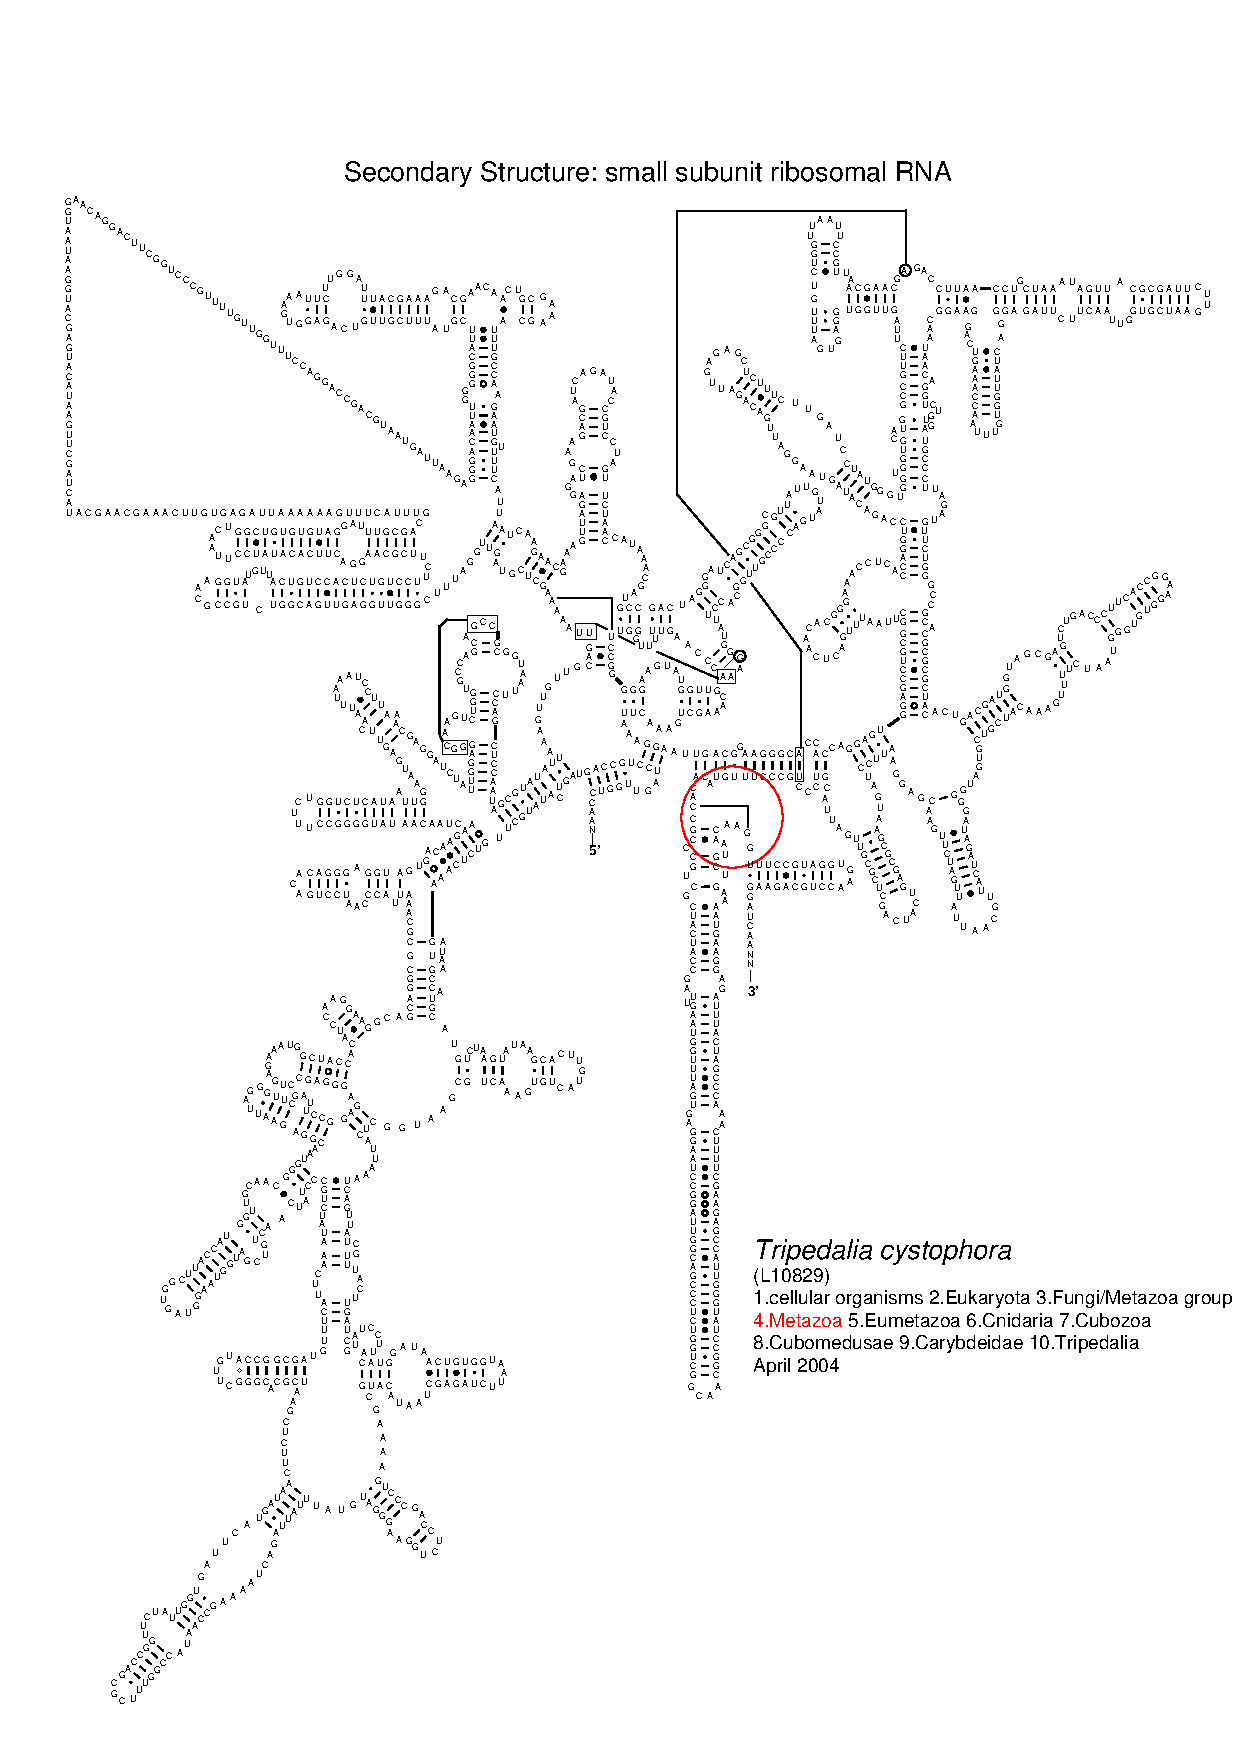
\includegraphics[width=0.45\textwidth]{../img/chyby/tripedalia_cystophora}
  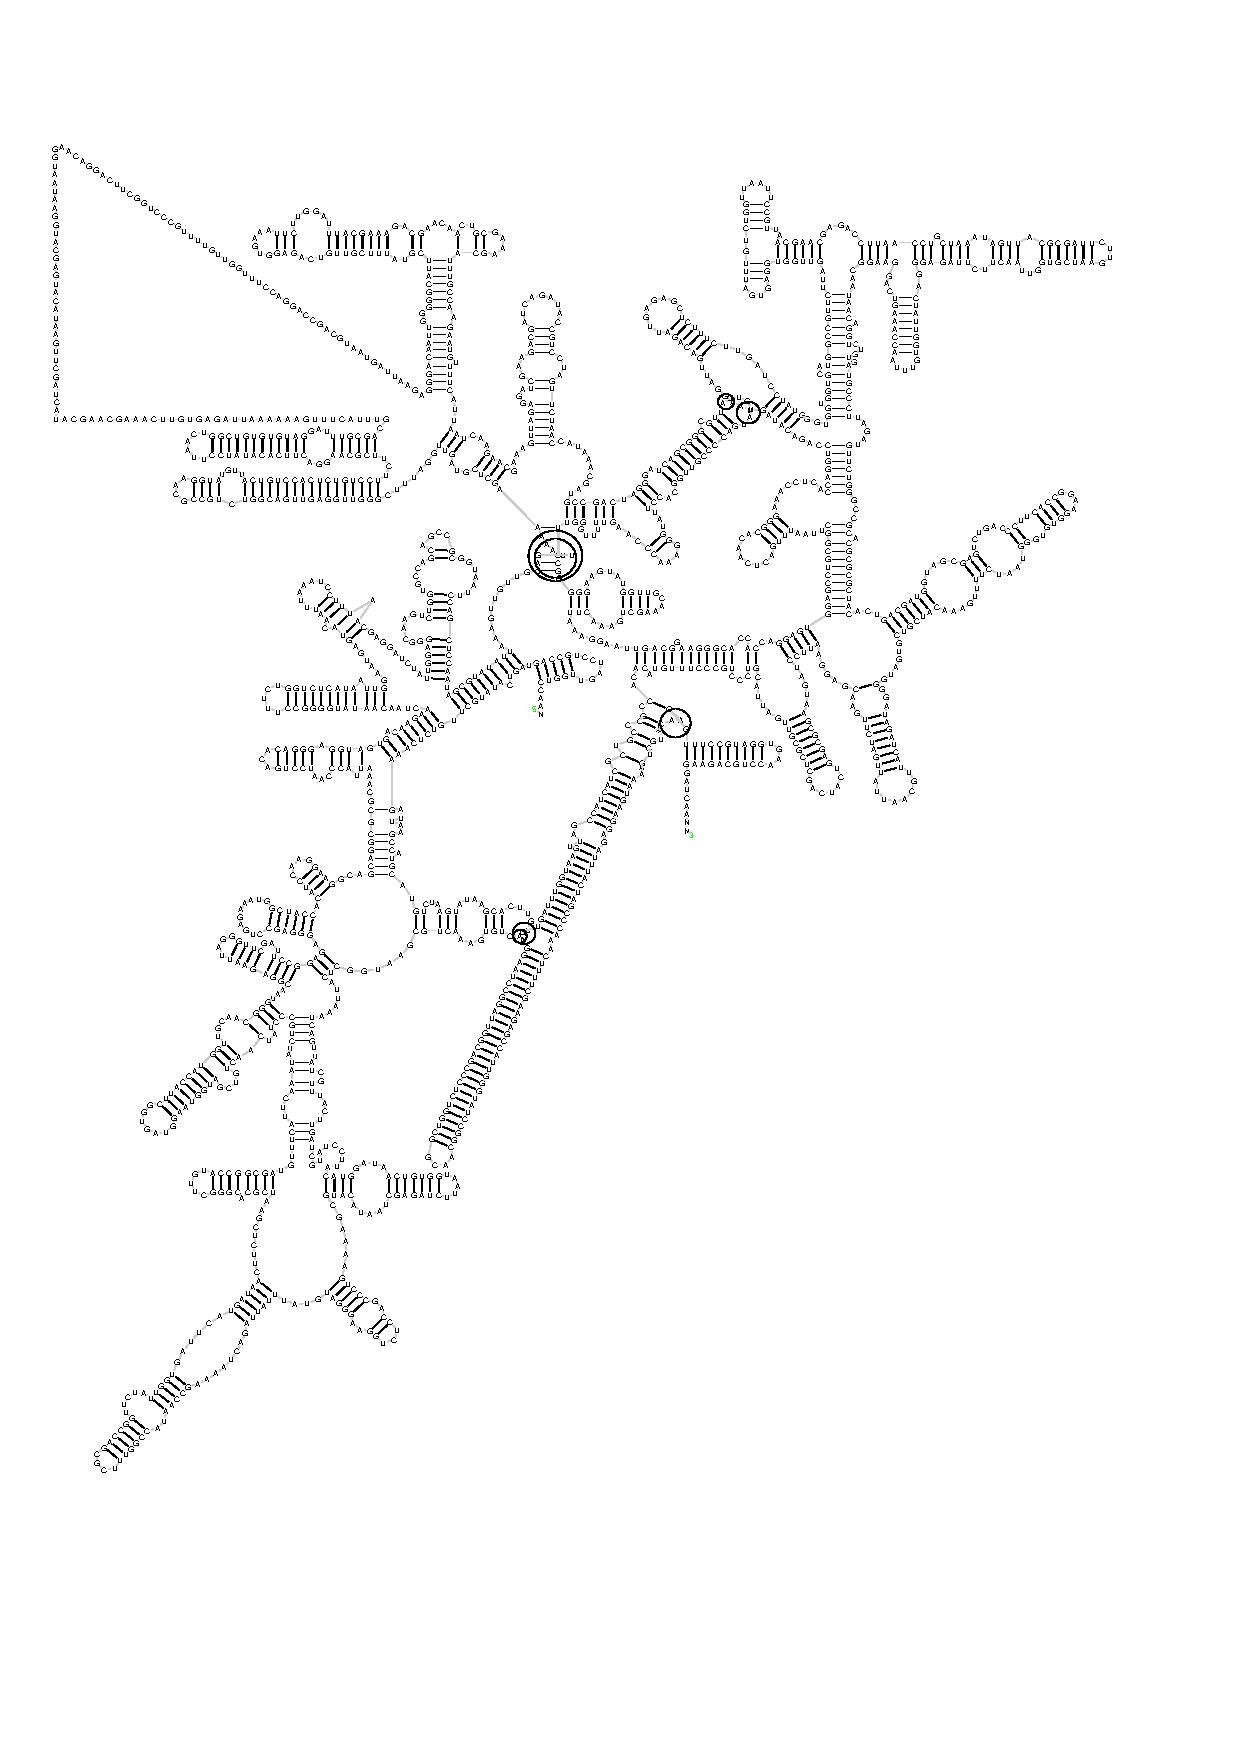
\includegraphics[width=0.45\textwidth]{../img/chyby/tripedalia_cystophora-tripedalia_cystophora}
  \caption{Chyba pri otočení vetvy}
  \label{obr:chyba_otočenie_vetvy}
\end{figure}

\subsection{Rozloženie báz na kružnicu}

Niekedy sa prekresleniu celej loop nevyhneme. Ak napríklad vkladáme veľmi veľké množstvo báz na jedno
miesto, dochádza k problémom načrtnutým na obrázku \ref{obr:chyba_rozloženie_loopy}.

Na tomto konkretnom príklade je nakreslený stem, vo vnútri ktorého je veľka loop. Kvoli tomu,
že chceme dodržiavať pravidlá o kružnicovom tvare loopy, nájdeme kružnicu dostatočne veľkú.
V tomto prípade až príliž veľkú.

Poznámka - vo vrchnej vetve ja taktiež znázornená kružnica, ale na rozdiel od spodnej obsahuje iba 2 vrcholy.

\begin{figure}[H]
%trim=left bottom right top
  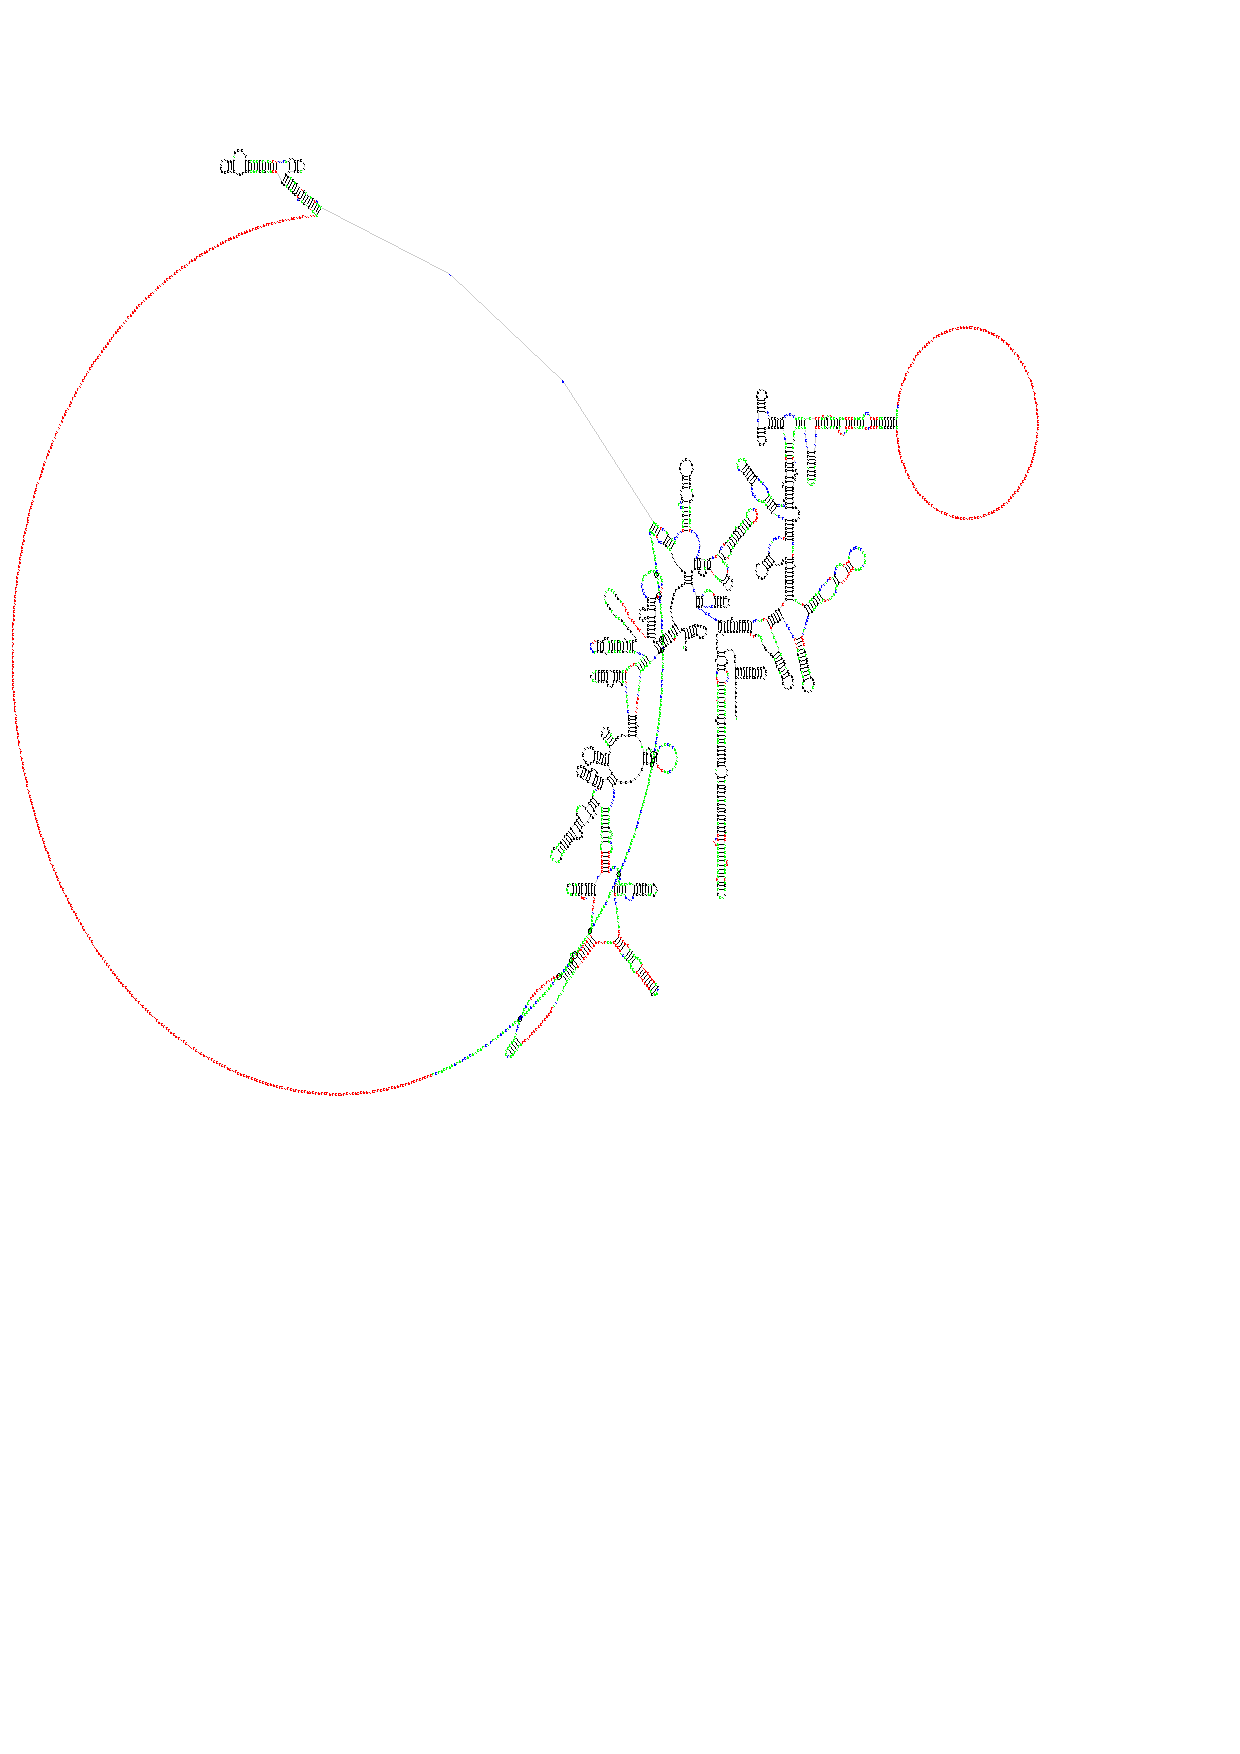
\includegraphics[clip, trim=0 10cm 3cm 2cm,width=0.8\textwidth]{../img/chyby/african_frog-echinococcus_granulosus}
  \caption{Chyba pri rozkladaní báz na kružnicu}
  \label{obr:chyba_rozloženie_loopy}
\end{figure}

\subsection{Otáčanie vetvy kvôli prekreslovaniu multibranch loopy}

Ako už aj graf na obrázku \ref{obr:štatistika_prekryvy_bez_rotacií} ukázal,
prekreslovanie multibranch loopy a rotácie všetkych vetiev spôsobuje masívne prekryvy.

Pripájame jeden priklad na obrázku \ref{obr:chyba_rotácia_multibranch}. Miesto vľavo dolu, kde začínajú
bázy sa sfarbovať na hnedo, je multibranch loop, ktorú sme potrebovali z dôvodu vloženej novej vetvy
(označená červeno) prekresliť.

Výsledok je taký, že všetky vetvy sme uložili na kružnicu a pootáčali do vhodného smeru a tým vzniklo
veľa prekryvov.

Na obrázku je vidieť ešte jednu vec, označené kríženia vo výslednom obrázku vľavo hore.
V kapitole o úpravach multibranch loop sme spomínali, že prekresleniu celej loopy sa snažíme
vyhnúť ak to ide. Predpokladáme, že ak je báz veľa a zmeny malé, bázy trochu poposúvame aby sa
nový vrchol zmestil medzi ne, alebo práve naopak ich roztiahneme, aby sme vyplnili medzeru po starom.
Kvôli tomu vyzerá táto štruktúra tak pomiešane a kvôli tomu na tomto mieste vznikajú ďalšie prekryvy.

\begin{figure}
  %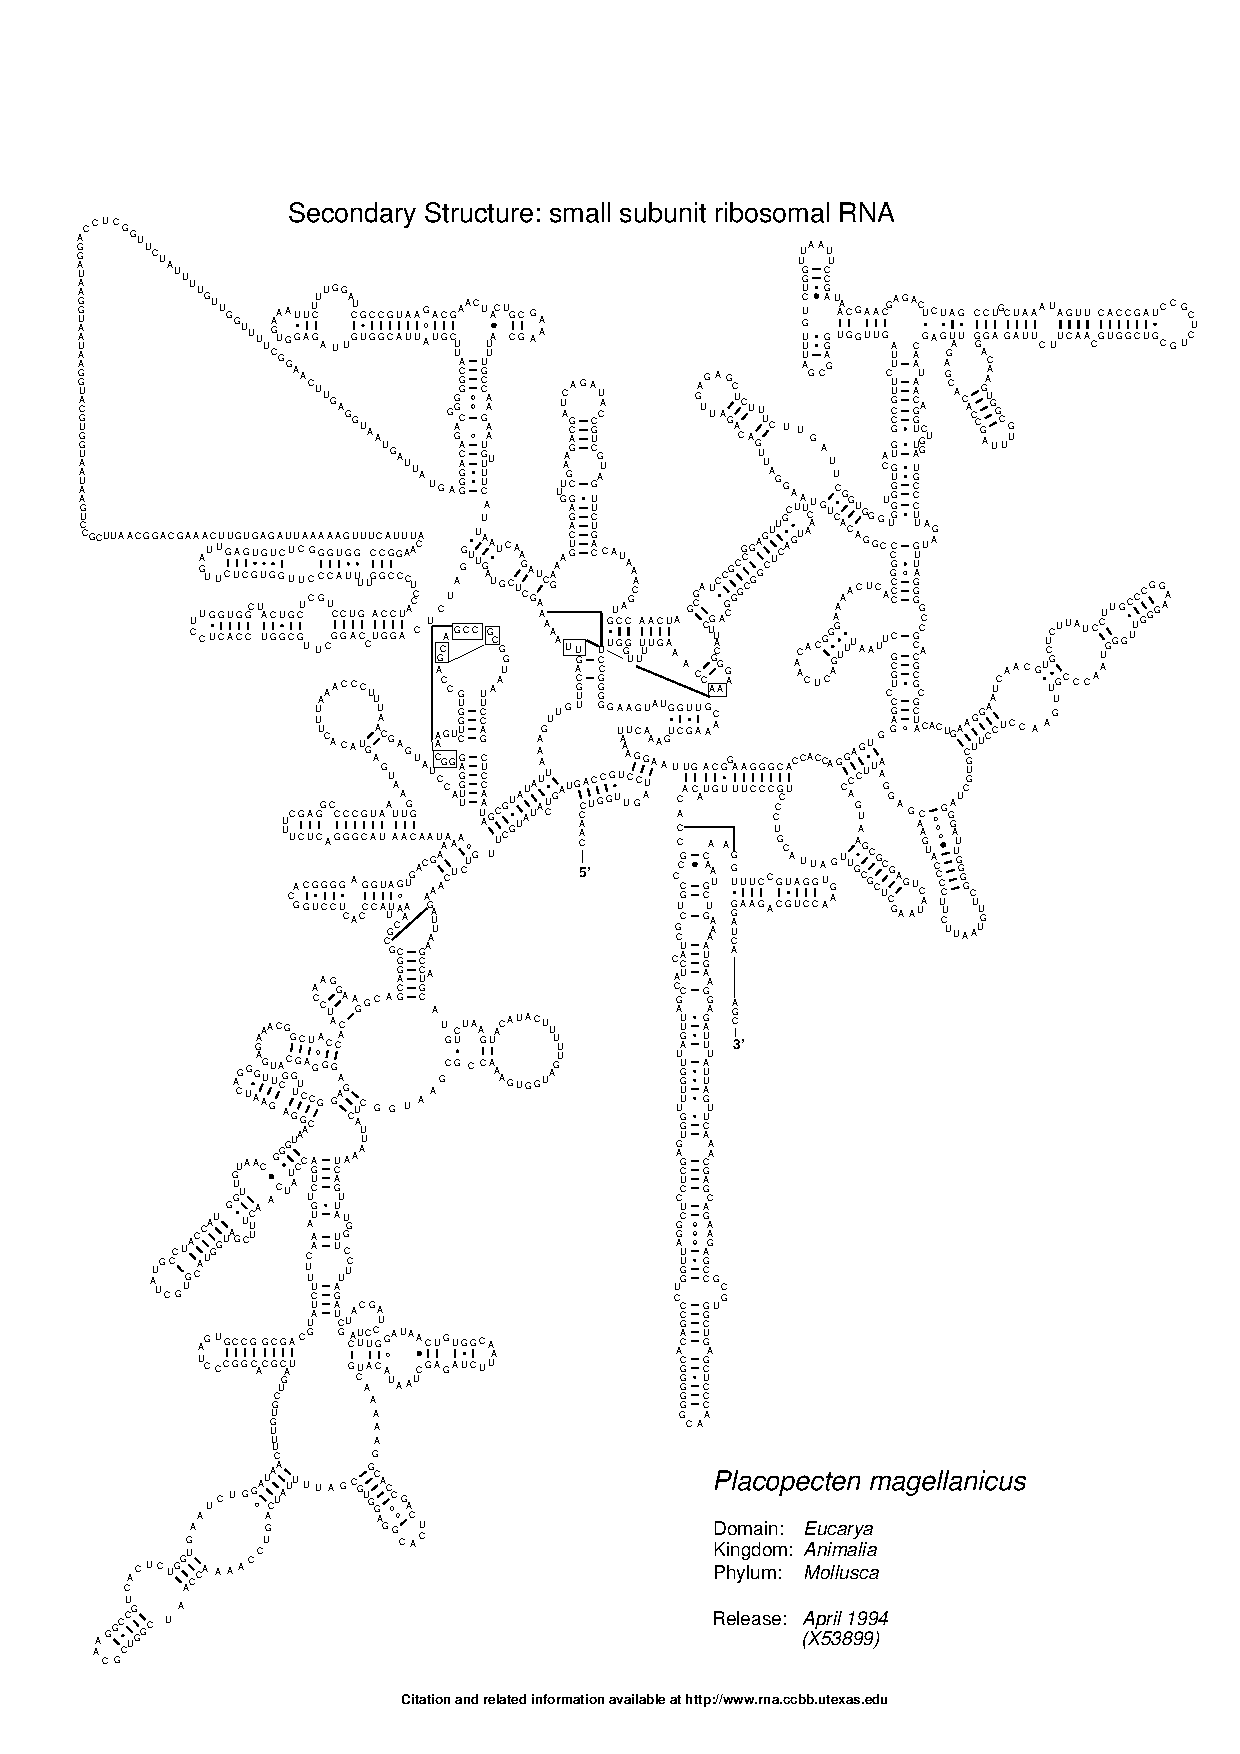
\includegraphics[width=0.45\textwidth]{../img/chyby/sea_scallop}
  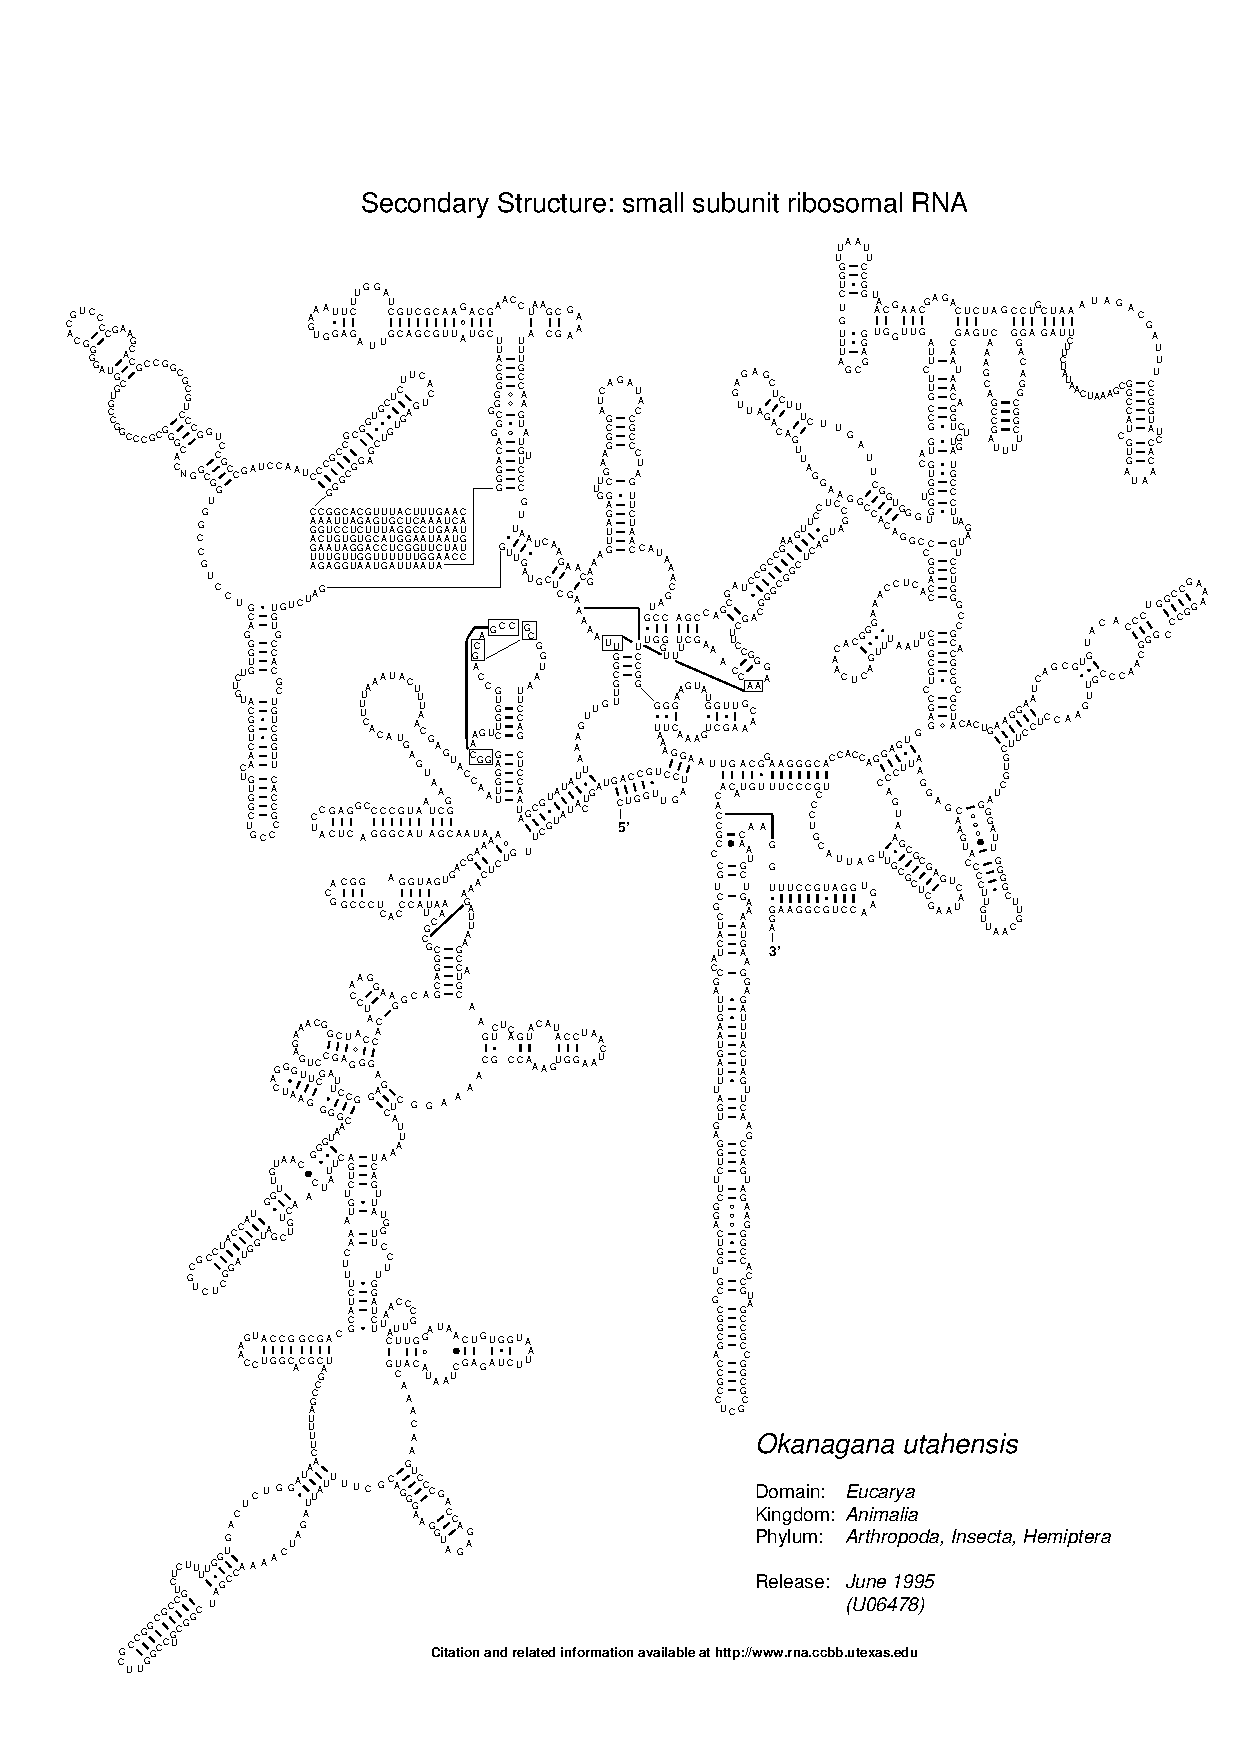
\includegraphics[width=0.45\textwidth]{../img/chyby/cicadas}
%trim=left bottom right top
  %\centering
  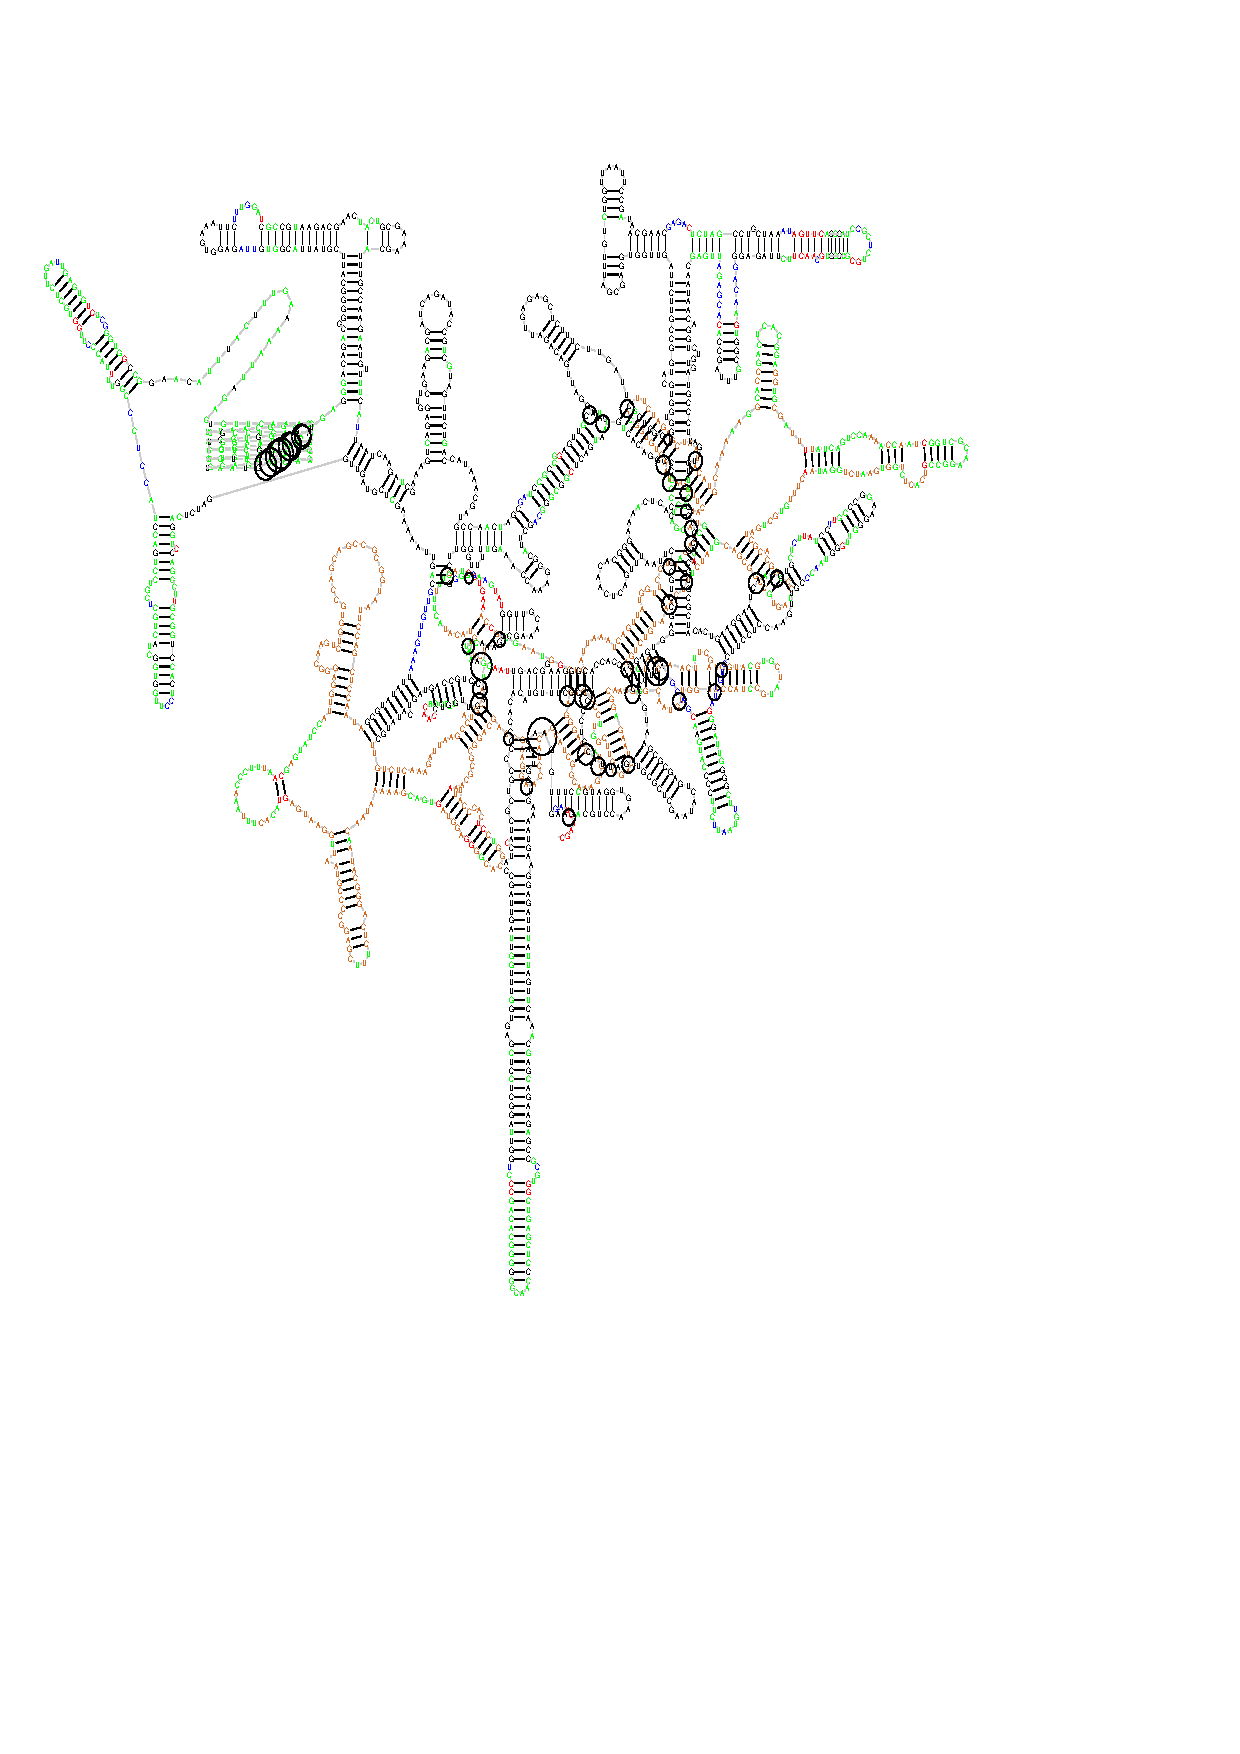
\includegraphics[clip, trim=0.5cm 7cm 4cm 2cm,width=0.45\textwidth]{../img/chyby/cicadas-sea_scallop}
  \caption{Chyba pri otáčani kvôli prekreslovaniu multibranch loopy}
  \label{obr:chyba_rotácia_multibranch}
\end{figure}









